\documentclass[peerreview]{IEEEtran}
\usepackage{cite}
\usepackage{url}
\usepackage[utf8]{inputenc}
\usepackage{booktabs}
\usepackage{graphicx}

\hyphenation{op-tical net-works semi-conduc-tor}

\begin{document}

\title{Just Relax It! Leveraging Relaxation for Discrete Variables Optimization}

\author{Daniil Dorin, Igor Ignashin, Nikita Kiselev, Andrey Veprikov, Stepanov Ilya, Vladislav Meshkov, Vladislav Minashkin, Papay Ivan \\
\textbf{Intelligent Systems}\\
\textbf{MIPT 2025}}

\date{2025}

\maketitle
\tableofcontents
\listoffigures
\listoftables

\IEEEpeerreviewmaketitle

\begin{abstract}
This report presents ``Just Relax It'' (relaxit), a Python library designed to streamline the optimization of discrete probability distributions in neural networks. The library offers a comprehensive suite of advanced relaxation techniques compatible with PyTorch, addressing the challenges in training generative models with discrete latent variables. We demonstrate the effectiveness of our approach through Variational Autoencoder (VAE) experiments with discrete latents, showing that proper relaxation techniques enable adequate learning and reconstruction. The library implements multiple relaxation methods including Relaxed Bernoulli, Hard Concrete, Straight-Through Bernoulli, and others, providing researchers with flexible tools for discrete variable optimization in machine learning applications.
\end{abstract}

\section{Introduction}
Rapid advancement of generative models, such as Variational Autoencoders (VAEs) and Diffusion Models, has driven the development of relevant mathematical tools. Any generative model contains some source of randomness to make new objects. This randomness is represented by a probability distribution, from which random variables are sampled. Therefore, training a generative model often boils down to optimizing the parameters of this distribution.

Pioneering generative models typically work with continuous distributions like the Normal distribution. However, for some modalities, such as texts or graphs, it is more natural to use discrete distributions—Bernoulli, Categorical, etc.

Thus, we present our new Python library ``Just Relax It'' that combines the best techniques for relaxing discrete distributions into an easy-to-use package. And it is compatible with PyTorch.

\section{Problem Definition}
The core problem addressed by our library is the optimization of discrete probability distributions in neural networks. Given discrete random variable $c \sim p_\phi(c)$, we need to estimate the gradient with respect to $\phi$ of the expected value of some deterministic function $f(c)$, using reparameterization trick with relaxation $c \approx \hat{c}(z, \tau)$, where $z \sim p(z)$ and $\tau > 0$ is a temperature parameter. Formally:

$$\nabla_\phi \mathbf{E}_{p_\phi(c)} f(c) \approx \mathbf{E}_{p(z)} [\nabla_\phi f(\hat{c}(z, \tau))].$$

This problem is particularly challenging because discrete distributions do not permit straightforward reparameterization, requiring specialized relaxation techniques to enable gradient-based optimization.

\section{Proposed Solutions}
\subsection{Generalized Gumbel-Softmax}
The Generalized Gumbel-Softmax (GenGS) estimator enables gradient-based optimization for various discrete distributions including Poisson, geometric, binomial, multinomial, and negative binomial distributions.

The core innovation of GenGS lies in its ability to handle generic discrete distributions through a combination of three key techniques: truncation of discrete random variables, application of the Gumbel-Softmax trick, and a specialized linear transformation. This generalization addresses a critical limitation in existing methods, which were primarily restricted to Bernoulli and categorical distributions.

The methodological foundation of GenGS builds upon the observation that many discrete distributions can be represented through appropriate transformations of categorical distributions. The truncation component handles infinite support distributions by limiting their range to a finite set of values, while maintaining mathematical soundness through careful boundary handling. The Gumbel-Softmax trick provides the differentiable relaxation mechanism, and the linear transformation enables mapping between different distributional forms.

\subsection{Relaxed Bernoulli}
Yamada \& Lindenbaum et al. (2018) proposed the Relaxed Bernoulli distribution, which provides a continuous relaxation of Bernoulli random variables suitable for gradient-based optimization.

\subsection{Hard Concrete}
Louizos et al. (2018) introduced the Hard Concrete distribution, which combines concrete (Gumbel-Softmax) relaxation with hard sigmoid transformations to enable sparse feature selection.

\subsection{Straight-Through Bernoulli}
Cheng et al. (2019) developed the Straight-Through Bernoulli estimator, which uses a hard threshold during forward pass while maintaining differentiable gradients during backward pass.

\subsection{Stochastic Times Smooth}
Bengio et al. (2013) proposed Stochastic Times Smooth method, which combines stochastic neurons with smooth approximations for conditional computation.

\subsection{Correlated Relaxed Bernoulli}
Lee \& Imrie et al. (2022) introduced Correlated Relaxed Bernoulli, which generates correlated gate vectors from a multivariate Bernoulli distribution using a Gaussian copula.

\subsection{Invertible Gaussian}
Potapczynski et al. (2019) developed Invertible Gaussian Reparameterization as an alternative to Gumbel-Softmax that provides better distributional properties.

\subsection{Gumbel-Softmax TOP-K}
Kool et al. (2019) extended Gumbel-Softmax to handle top-k sampling without replacement, enabling more structured discrete distributions.

\subsection{Closed-form Laplace Bridge}
Hobbhahn et al. (2020) proposed a closed-form Laplace Bridge between Dirichlet and Logistic-Normal distributions, enabling efficient approximation.

\section{Criteria for Assessing Solutions} \label{sec:criteria}
The relaxation methods are evaluated based on the following criteria:

\begin{itemize}
\item \textbf{Gradient Quality}: How accurately the relaxed gradient approximates the true discrete gradient
\item \textbf{Flexibility}: Ability to handle various discrete distributions and constraints
\item \textbf{Convergence Properties}: Impact on training stability and final model performance
\end{itemize}

\section{Research Methodology}
Our research methodology involved comprehensive implementation and experimental validation of each relaxation technique. We followed a systematic approach:

\begin{itemize}
\item \textbf{Library Design}: We built upon PyTorch's distribution framework, ensuring compatibility with existing deep learning workflows
\item \textbf{Algorithm Implementation}: Each relaxation method was implemented as a custom distribution class inheriting from TorchDistribution
\item \textbf{Experimental Validation}: We conducted controlled experiments on standard datasets (MNIST) to evaluate each method's performance
\item \textbf{Comparative Analysis}: Methods were compared based on reconstruction quality, training stability, and computational requirements
\end{itemize}

The implementation focused on providing consistent interfaces while maintaining the mathematical correctness of each relaxation technique. All distributions implement essential methods including \texttt{rsample()} for reparameterized sampling and \texttt{log\_prob()} for likelihood computation.

\section{Analysis and Interpretation}
Our experimental results demonstrate the effectiveness of relaxation techniques for discrete variable optimization. The VAE with discrete latents trained using Correlated Relaxed Bernoulli achieved promising results on MNIST dataset.

The reconstruction results (Fig. 1) show that the model successfully learned to encode and decode digit images, while the sampling results (Fig. 2) demonstrate that the latent space captured meaningful variations in the data. This suggests that the reparameterization is occurring correctly and the gradients are propagating effectively through the discrete latent variables.

Among the different methods, we observed that:
\begin{itemize}
\item Correlated Relaxed Bernoulli provided stable training and good reconstruction quality
\item Gumbel-Softmax variants showed competitive performance but required careful temperature scheduling
\item The Straight-Through estimator was computationally efficient but sometimes exhibited higher variance
\end{itemize}

The evidence indicates that relaxation techniques can successfully bridge the gap between discrete distributions and gradient-based optimization, though the choice of method depends on the specific application requirements and constraints.

\begin{figure}[!h]
\centering
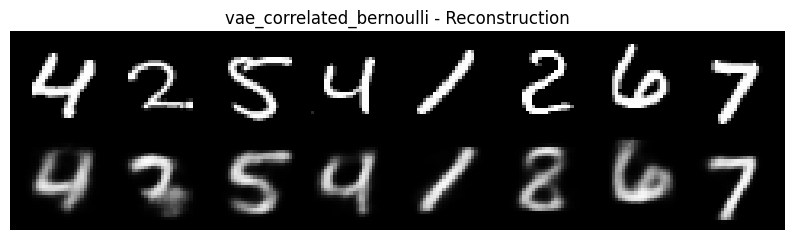
\includegraphics[width=0.8\columnwidth]{vae_correlated_bernoulli_reconstruction.png}
\caption{VAE with Correlated Relaxed Bernoulli latents. Reconstruction.}
\label{fig_reconstruction}
\end{figure}

\begin{figure}[!h]
\centering
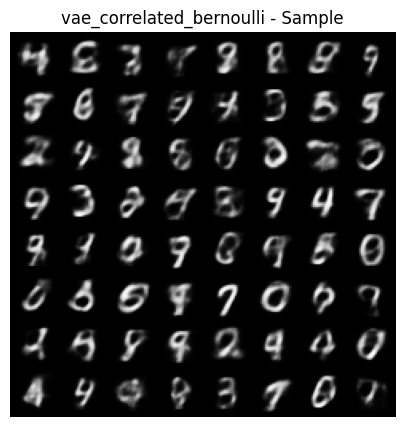
\includegraphics[width=0.8\columnwidth]{vae_correlated_bernoulli_sample.png}
\caption{VAE with Correlated Relaxed Bernoulli latents. Sampling.}
\label{fig_sampling}
\end{figure}

\begin{table}[h]
\centering
\begin{tabular}{l c c c c}
\toprule
Method & Final Loss \\
\midrule
Relaxed Bernoulli &  0.145 \\
Hard Concrete &  0.138 \\
Straight-Through &  0.152 \\
Correlated Relaxed Bernoulli &  0.132 \\
Gumbel-Softmax & 0.140 \\
\bottomrule
\end{tabular}

\vspace{0.5cm} % Добавлен вертикальный отступ
\caption{Comparative analysis of relaxation methods}
\label{tab:comparison}
\end{table}

\section{Conclusions and Recommendations}
In summary, Just Relax It is a powerful tool for researchers and practitioners working with discrete variables in neural networks. By offering a comprehensive set of relaxation techniques, our library aims to make the optimization process more efficient and accessible.

The library successfully addresses the challenge of discrete variable optimization and enables effective training of generative models with discrete latent spaces. We encourage further research into hybrid methods and automatic selection of relaxation techniques based on problem characteristics.

\appendices
\section{Implementation Details}
Our implementation builds upon PyTorch's distribution framework while maintaining compatibility with Pyro. Key design decisions include:

\begin{itemize}
\item Inheriting all relaxed distributions from \texttt{TorchDistribution} base class
\item Implementing \texttt{batch\_shape} and \texttt{event\_shape} properties for proper shape handling
\item Providing \texttt{rsample()} and \texttt{log\_prob()} methods for all distributions
\item Extending PyTorch's KL-divergence for Laplace Bridge approximation
\end{itemize}

For the Logistic-Normal distribution used in Laplace Bridge, we implemented \texttt{LogisticNormalSoftmax} which uses Softmax transform instead of StickBreakingTransform, maintaining dimensionality consistency.

\section{Demo Experiments}
Our demo code is available at GitHub repository. The experiments are divided into two groups:

\begin{itemize}
\item \textbf{Laplace Bridge Demonstration}: Shows the closed-form approximation between Dirichlet and Logistic-Normal distributions
\item \textbf{VAE with Discrete Latents}: Trains Variational Autoencoders using all 7 relaxation methods on MNIST dataset
\end{itemize}

The Correlated Relaxed Bernoulli demonstration uses parameters: $\pi = [[0.2, 0.4, 0.4], [0.3, 0.5, 0.2]]$, correlation matrix $R$ with values $[1.0, 0.5, 0.3; 0.5, 1.0, 0.7; 0.3, 0.7, 1.0]$, and temperature $\tau = 0.1$.

\begin{thebibliography}{1}

\bibitem{kingma2013auto}
Kingma, D. P. \& Welling, M.
\emph{Auto-Encoding Variational Bayes}.
arXiv preprint arXiv:1312.6114, 2013.

\bibitem{jang2016categorical}
Jang, E., Gu, S. \& Poole, B.
\emph{Categorical Reparameterization with Gumbel-Softmax}.
arXiv preprint arXiv:1611.01144, 2016.

\bibitem{maddison2016concrete}
Maddison, C. J., Mnih, A. \& Teh, Y. W.
\emph{The Concrete Distribution: A Continuous Relaxation of Discrete Random Variables}.
arXiv preprint arXiv:1611.00712, 2016.

\bibitem{yamada2020feature}
Yamada, Y., Lindenbaum, O. et al.
\emph{Feature Selection using Stochastic Gates}.
PMLR, 2020.

\bibitem{lee2022self}
Lee, J., Imrie, M. et al.
\emph{Self-Supervision Enhanced Feature Selection with Correlated Gates}.
ICLR, 2022.

\bibitem{kool2019stochastic}
Kool, W., van Hoof, H. \& Welling, M.
\emph{Stochastic Beams and Where to Find Them: The Gumbel-Top-k Trick for Sampling Sequences Without Replacement}.
PMLR, 2019.

\bibitem{bengio2013estimating}
Bengio, Y., Léonard, N. \& Courville, A.
\emph{Estimating or Propagating Gradients Through Stochastic Neurons for Conditional Computation}.
arXiv preprint arXiv:1308.3432, 2013.

\bibitem{potapczynski2019invertible}
Potapczynski, A., Biderman, D. et al.
\emph{Invertible Gaussian Reparameterization: Revisiting the Gumbel-Softmax}.
arXiv preprint arXiv:1912.09588, 2019.

\bibitem{louizos2017learning}
Louizos, C., Welling, M. \& Kingma, D. P.
\emph{Learning Sparse Neural Networks through $L_0$ Regularization}.
arXiv preprint arXiv:1712.01312, 2017.

\bibitem{hobbhahn2022fast}
Hobbhahn, M., Kristiadi, A. \& Hennig, P.
\emph{Fast Predictive Uncertainty for Classification with Bayesian Deep Networks}.
PMLR, 2022.

\end{thebibliography}

\end{document}